\chapter{Datenvisualisierung}
\label{ch:data_visualization}

Die Visualisierung von Ergebnissen ist der wichtigste Aspekt einer Anwendung. Der Nutzer will die Ergebnisse einfach und schnell erkennen können. Hierzu hängt die Art und Weise der Visualisierung sehr stark von den Daten und ihren Ergebnissen ab. Im forensischen Umfeld geht es um die Visualisierung von großen Datenmengen und dem Auffinden der sprichwörtlichen \textit{Nadel im Heuhaufen}. Daher ist es umso wichtiger passende Werkzeuge bereitzustellen, um die Daten nach bestimmten Kriterien filtern zu können. Darüber hinaus muss es möglich sein, die Dateiinhalte (Bilder, Videos und  Dokumente) schnell und zuverlässig anzeigen zu können.\\

\noindent
Im Vergleich hierzu bietet die Referenzsoftware \textit{Autopsy} eine gute Möglichkeit zur Datenvisualisierung. So besteht die Möglichkeit die Dateien einzelner Datenträger in einer hierarchischen Sicht zu durchsuchen. Es existieren auch sogenannte \textit{Views}, um alle Bilder oder alle gelöschte Dateien anzuzeigen. Ein wichtiger Aspekt ist auch die Analyse der Zeitstempel. Hierzu existiert eine eigene Ansicht mit einer Zeitleiste, um nach Ereignissen in einem bestimmten Zeitraum zu suchen. Es besteht auch eine Möglichkeit Kommunikationswege aufgrund von gesendeter E-Mails und besuchten Websites zu visualisieren. Autopsy bietet hier eine breite Auswahl, wie Daten gefiltert und analysiert werden können.\\

\noindent
Für die hier entwickelte forensische Analyseplattform kann die Datenvisualisierung als Web-Applikation implementiert werden. Der Zugriff auf die forensischen Rohdaten kann über Apache Solr durchgeführt werden, da die indexierten Daten über eine REST-Schnitt-stelle zu Verfügung gestellt werden.\footnote{Siehe auch Kapitel \ref{sec:theory_solr}.}\\

\noindent
In einer Testimplementierung wird eine rudimentäre Oberfläche zur Anzeige und Filterung der Metadaten entwickelt. Hierzu wird das Open-Source Projekt \textit{Banana} genutzt, um die in Solr indexierten Daten zu visualisieren.\footnote{Siehe Link: \url{https://github.com/lucidworks/banana}. Letzter Zugriff: 23.8.2018.} Banana basiert auf dem weit verbreiteten Analyse-Framework \textit{Kibana}, welches die indexierten Daten von Elasticsearch visualisieren kann.\footnote{Siehe Link: \url{https://www.elastic.co/products/kibana}. Letzter Zugriff: 24.9.2018.} Analog hierzu stellt Banana einzelne UI-Komponenten bereit, um die Daten aus Solr zu visualisieren. Obwohl das Projekt nicht mehr gepflegt wird, so zeigt es doch wie simpel und performant die Daten aus Solr über die REST-Schnittstelle abgefragt und visualisiert werden können.\footnote{Der letzte Commit im Repository auf Github erfolgte im Juni 2017. Daher wird das Projekt sehr wahrscheinlich nicht mehr weiter gepflegt.}
Abbildung \ref{fig:banana_visualization} zeigt die Datenvisualisierung mit Banana.

\begin{figure}[ht]
  \centering
  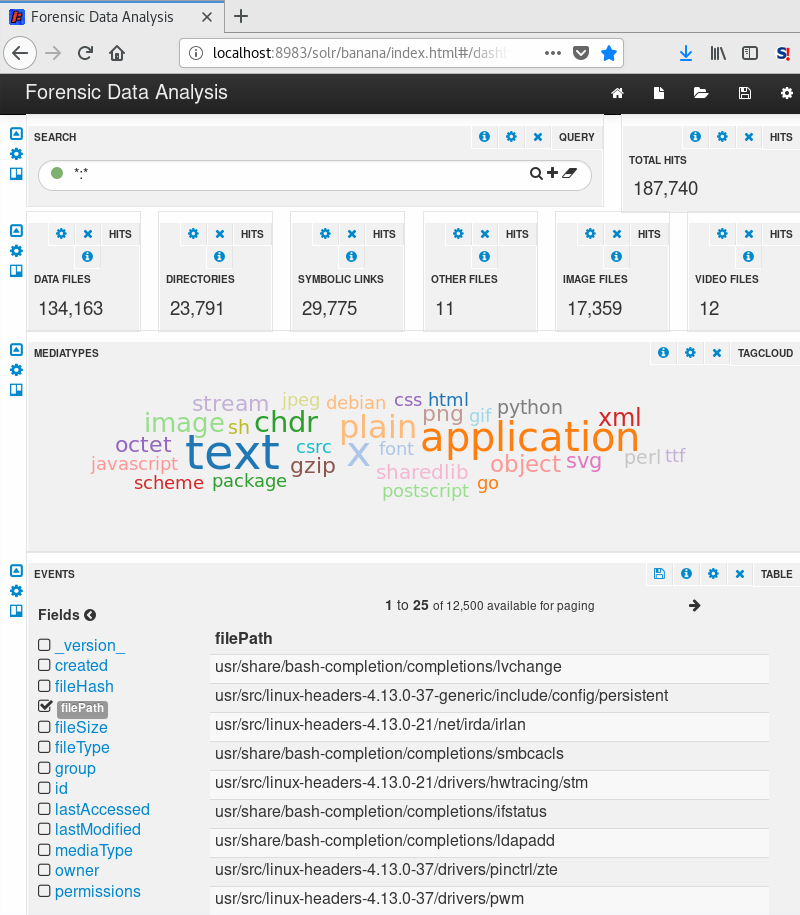
\includegraphics[width=0.9\textwidth]{./resource/forensicDataAnalysisUI.png}
  \caption{Visualisierungsbeispiel mit Banana}
  \label{fig:banana_visualization}
\end{figure}

\noindent
Die Oberfläche ist in mehrere Komponenten aufgeteilt. Die erste Komponente ist die Volltextsuche, die es ermöglicht in den Metadaten nach bestimmten Wörtern und Werten zu suchen. In der zweiten Zeile befinden sich diverse Statistiken, die bei jeder Filterung oder Suche aktualisiert werden. 
Im aktuellen Beispiel werden alle importierten Daten angezeigt. Dies sind insgesamt 187.740 Dateien. Darunter sind 134.163 Datendateien und 23.791 Verzeichnisse. In den Daten wurden 17.359 Bilder und 12 Videos erkannt. Diese Werte basieren auf der Datenauswertung der Medientypen, welche bei der Datenverarbeitung ermittelt wurden (siehe Kapitel \ref{subsec:media_types}).\\
In der dritten Zeile werden die 30 häufigsten vorkommenden Medientypen in einer sogenannten \textit{Word Cloud} angezeigt. In der vierten Zeile hingegen werden die Ergebnisse der Suchanfrage angezeigt. Im konkreten Fall werden einfach die ersten beliebigen Dateien angezeigt. 
Sobald der Analyst aber beispielsweise nach einem bestimmten Dateinamen sucht, werden alle Dateien mit diesem Namen in der Ergebnisliste ausgegeben. Zusätzlich können einzelne Attribute visualisiert werden.\\
Mit Banana ist es auch möglich die Dateizeitstempel auszuwerten und danach zu filtern.\\

\noindent
Gerade auch im Open-Source Bereich existieren noch weitere Projekte, welche zukünftig für eine Datenvisualisierung genutzt werden könnten. So wäre es möglich, komplexe Zusammenhänge in der Graphendatenbank \textit{Neo4j} zu speichern und deren Graphenvisualisierung in die Web-Applikation zu integrieren.\footnote{Siehe Link: \url{https://neo4j.com/}. Letzter Zugriff: 24.9.2018.} Zur Erstellung weiterer Datenvisualisierungen könnten auch die Projekte \textit{Grafana}\footnote{Siehe Link: \url{https://github.com/grafana/grafana}. Letzter Zugriff: 24.9.2018.} oder \textit{Apache Superset}\footnote{Siehe Link: \url{https://github.com/apache/incubator-superset}. Letzter Zugriff: 24.9.2018.} genutzt werden.\\
Auch die JavaScript Bibliothek \textit{D3.js} bietet dutzende Arten zur Datenvisualisierung, welche im forensischen Umfeld bei großen Datenmengen genutzt werden könnten.\footnote{Siehe Link: \url{https://d3js.org/}. Letzter Zugriff: 24.9.2018.}\\


% Wordcloud, geographische Visualisierung, Flare-Chart, Tree-Map, Calendar-Chart als Timeline?
% Webframeworks wie \url{https://d3js.org/} \footnote{Siehe Links: \url{https://bl.ocks.org/mbostock/4063550}, \url{https://bl.ocks.org/mbostock/5944371}, \url{https://bl.ocks.org/mbostock/1046712}, \url{https://bl.ocks.org/mbostock/4063269} und \url{http://xliberation.com/googlecharts/d3concept.html}. Letzter Zugriff: 25.7.2018}
% Open Source Community Variante Helical Insight
% Apache Superset für Visualisierung (siehe Ambari Cluster Services)
% Apache Grafana?
% GoJs incremental tree?
% Druid.io

%Duplicate Flag in DB schreiben, um über Banana UI alle Duplikate finden zu können...